

\chapter{Multi-episodic Perceived Quality in Multiple Days}\label{chap:field}
%\begin{chapter-abstract}
%Here I present all studies that I conducted on multi\-/episodic QoE over several days.
%This will include studies with one service only, but also with two services (multi-service) part.
%
%\textit{Key question:} do field trials (longer timespan) yield similar effects as found in lab trials (chap 6).
%What are the differences? (If there are any)
%What services are technically feasible to deploy (or socially manageable)?
%How to conduct a study over several days (lab vs. field)?
%
%The main study will be the currently \textit{successfully} running Audio-on-demand study with BYOD.
%This study is complemented by QoMEX2014 study.
%This chapter will also include an overview of limitations and practical knowledge for \textit{successful} field trials.
%
%%TODO: \section{Digression: Retaining Information}%Can subjects recall
%\end{chapter-abstract}

%\section{Introduction}


The integration of perceived quality of usage episodes into a multi\-/episodic perceived quality is not limited to one session alone.
Rather usage episodes with a service often occur regularly and might cover multiple days or even longer usage periods.
In difference to consecutive usage in one session, the time that passes between episodes might be longer.
However, it is so far unknown how and if at all the time between episodes affects the quality formation process of multi\-/episodic perceived quality.
%Due to the lack of ground truth, the findings for one session (\cf{} \autoref{chap:lab}) are used as a basis towards this investigation.
A feasible option to cover such time spans in an experiment is to conduct it as a field experiment.
Here, field experiment refers to a subjective experiment conducted with participants in their home environment over several days.
This enables repeated-use of a service for rather short episodes while limiting the effort for participants.
However, this approach has two inherent limitations.
First, the usage environment cannot be controlled and is unlikely to be identical between participants.
Second, participants cannot be directly supervised during the experiment.
Both might be confounding factors.
In addition, technical systems must be robust while providing the desired performance level per usage episode.

For the investigation of multi\-/episodic perceived quality with a usage period of multiple days, three experiments were conducted denoted as \E4{}, \E5{}, and \E6{}.
These experiments apply the defined-use method.
Following \citet{moller_single-call_2011}, each usage episode was presented individually, \ie, one episode per session.
\E4{} and \E5{} focused on general feasibility of investigating multi\-/episodic perceived quality in a field experiment.
These experiments covered a usage period of 14~days in which participants used two services on a daily basis.
Besides feasibility, \E4{} focused on the reproduction of the results of \citet{moller_single-call_2011}.
In \E5{}, the adaptation speed of multi\-/episodic judgments was planed to be investigated.
Based on \E4{}, \E5{}, and the one-session experiments, \E6{} was designed.
Here, \autoref{hypo:number}, \autoref{hypo:position}, and \autoref{hypo:consecutive} were investigated.
In this experiment only one service was used in a usage period of 6~days.

In all three experiments, two performance levels were applied.
These are also denoted as \ac{HP} and \ac{LP}.
Performance levels were applied day-wise, \ie, usage episodes on the same day with the same service were presented with the same performance level.
The performance levels were different between the three experiments.

\newcolumntype{Z}[1]{>{\centering\arraybackslash}p{#1}}
\label{E4}\label{E5}\label{E6}
\begin{table}[t]
	\centering
	\caption{Multiple days: overview on experiments.}
	\label{tab:field:experiments}
	\begin{tabulary}{\textwidth}{Z{1.3cm}|Z{2.3cm}|Z{3.4cm}|Z{1.2cm}|Z{1.5cm}}
	Experi-ment	& Service types 		& Tasks															& Days	& Partici-pants \\
	\midrule
	\E4{}		& Telephony	and \ac{VoD}	& Two-party conversation (\ac{SCS})	& 14		& 20\\ %Study 1/E4a
	\hline
	\E5{}		& \ac{VoD} and \ac{AoD}	& Audio book	and Video consumption		& 14		& 21 \\ %Study 3
	\hline
	\E6{}		& \ac{AoD}								& Audio book													& 7		& 95 %Study 14
	\end{tabulary}
\end{table}

\autoref{tab:field:experiments} gives an overview of the experiments including service types, tasks, and number of participants.
In the following, the experiments are presented one after the other.
The results are reported as \ac{MOS} ranging from 0~to~6 with standard deviation in brackets.
A statistical evaluation is conducted by applying the nonparametric tests as for the one-session experiments (\cf{} \autoref{method:statistic}).

\section{Experiment E4}
\E4{} was inspired by \citet{moller_single-call_2011}.\footnote{The results of \E4{} are published in \citet{guse_macro-temporal_2013}.}
The experiment of \citet{moller_single-call_2011} indicated only little differences for multi\-/episodic judgments between the evaluated multi\-/episodic conditions (\cf{} \hyperref[prior:moeller]{Section \ref*{prior:moeller}}).
This might be due to the limited number of degraded episodes or the introduced degradations were not severe enough.
The goal of \E4{} was the application of the defined-use method in a similar usage period to \citet{moller_single-call_2011} and to gather practical knowledge about how to conduct a field experiment.
In addition, conducting \E4{} had two goals:
First, a larger difference of multi\-/episodic judgments between conditions was desired to investigate the formation process.
For this \emph{a)} the number of \ac{LP} episodes was increased and \emph{b)} the performance parameters selected, so the perceptual difference between \ac{HP} and \ac{LP} was increased.
Second, two services were used.
This enabled to investigate the formation process in presence of two services.

\subsection{Design}
In this experiment, a speech telephony service and a \ac{VoD} service were selected.
The two services needed to be used daily over a usage period of 14~days.
The telephony service was used by a pair of participants together.
Each pair needed to solve two \acp{SCS} per day: the first one between \unit[6]{am} and \unit[1]{pm} and the second one between \unit[3]{pm} and midnight.
The \ac{VoD} service needed to be used daily for one episode between \unit[1]{pm} and midnight.
Here, \emph{Friends Season~3} episode 1..8 were used.
Each original episode was split into two parts while not disturbing the storyline.
The duration of these parts ranged from \unit[12]{min} to \unit[17]{min}.
For each usage episode one part was presented.

In this experiment, two conditions were investigated.
In the first one, all usage episodes were presented in \ac{HP} (denoted as \C0{}).
In the second condition, denoted as \C9{}, both services were presented in \ac{HP} for the first two days followed by two days \ac{LP} and so forth. \label{C9}
This resulted in 8~days presented \ac{HP} versus 6~days presented in \ac{LP}. 
While \C0{} replicates the baseline condition of \citet{moller_single-call_2011}, \C9{} should lead to a reduction in multi\-/episodic judgments.

After finishing an episode, participants assessed the episodic perceived quality on the 7\=/point \ac{CoCR} scale (\cf{} \autoref{img:chap05:quality-scale}).
The multi\-/episodic perceived quality for each service was assessed on the 4th, 7th, 10th, and 14th day directly after finishing the daily episode with the \ac{VoD} service (same scale).

For the speech telephony service, the speech codec \textsc{\lowercase{G.722}} was used with a packet length of \unit[20]{ms} for \ac{HP} and for \ac{LP}.
Neither \acs{FEC} nor elaborate algorithms for \acs{PLC} were applied.
For \acs{PLC}, only zero insertion was used.
For \ac{LP}, a random packet loss rate of 5\% was inserted in addition.
For the \ac{VoD} service, the video was encoded with \textsc{\lowercase{H.264}} at a resolution of \unit[720$x$576]{px} and the audio channel encoded with \acs{AAC} (\unit[48]{kHz}, \unit[165]{kbit/s}, stereo).
The two performance levels for this service differed only in the video encoding bandwidth.
For \ac{HP}, a bandwidth of \unit[2]{Mbit/s} and for \ac{LP} a bandwidth of \unit[125]{kbit/s} was applied.

In this experiment, participants used their own computer.
For audio reproduction and recording, a \emph{Logitech~PC120} headset was provided to each participant.
The speech telephony service was implemented as a \ac{VoIP} service, whereas the \ac{VoD} service was only simulated.
The latter only played local preprocessed content.
The video was always played in full screen independent of the actual screen size or resolution.
A complete description of the technical setup can be found in the \appendix{}~\ref{appendix:setups} (p.\,\pageref{appendix:setups}).

On the day before starting the 14~day usage period, an introductory session was conducted with each pair of participants.
In this session, participants received detailed instructions for this experiment and provided their demographic data.
Also, one episode with each of the two services need to be solved.
These were presented in \ac{HP}.
%This allowed that participants know how to use the two service and understood the necessary requirements for this experiment.
%Here also the \ac{NPS} was assessed for each service individually and for both services as a bundle.

\subsection{Participants}
\E4{} was conducted in Berlin, Germany from August to September~2012.
For each of the two conditions, 5~pairs successfully finished this experiment with an average age of 22.9~years ($\sigma = 3.1$), consisting of 11~male and 9~female participants.
Of the 280~scheduled calls, 5~were not conducted and 18~episodic judgments missing.
For the \ac{VoD} service, all episodes were conducted, but 13~episodic judgments and one multi\-/episodic judgment were missing.
This is, in fact, an issue with regard to the evaluation, \ie, deriving a \ac{MOS}, as desired by applying the defined-use method, because not all participants assigned to a multi\-/episodic condition were exposed to the same multi\-/episodic condition.
However, due to the small sample size and the missing ground truth, no participant was removed from the data analysis.

\subsection{Data Analysis}
First, the episodic judgments are evaluated for the \ac{VoD} service followed by a detailed analysis of the multi\-/episodic judgments.
An analysis of the speech telephony service is omitted here, as the implemented setup failed to provide the desired performance levels. 
Thus, a \ac{MOS} evaluation could not be conducted, as participants were not exposed to the same multi\-/episodic condition.
\autoref{img:field:E4conditionA1TELboxplot} shows the box plot for the episodic judgments for the \ac{VoD} service in \C9{}.
In the following, first the episodic judgments are analyzed followed by the analysis of the multi\-/episodic judgments.

\begin{figure}
	\centering
\begin{knitrout}
\definecolor{shadecolor}{rgb}{0.969, 0.969, 0.969}\color{fgcolor}
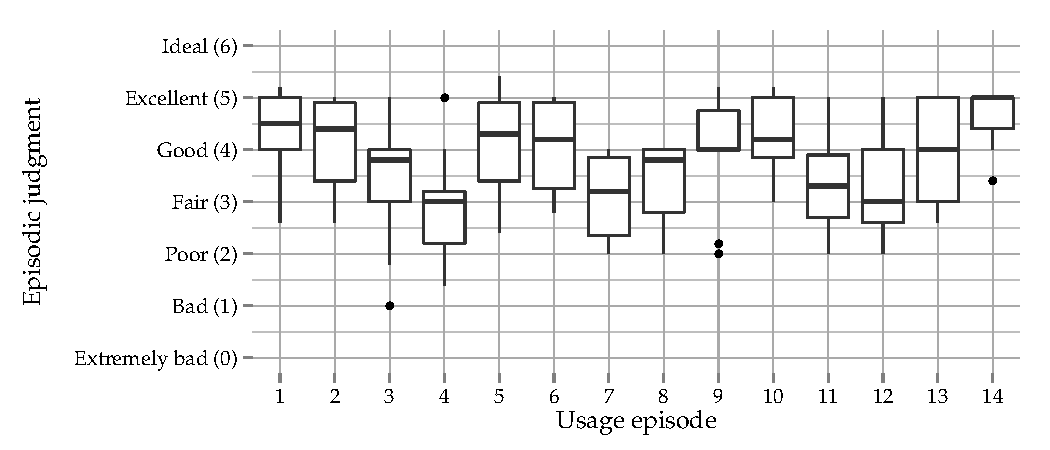
\includegraphics[width=\maxwidth]{figure/plotE4C0-1} 

\end{knitrout}
	\caption{Multiple days (\E4{}): episodic judgments for the \ac{VoD} service in \C9{}.}
	\label{img:field:E4conditionA1TELboxplot}
\end{figure}

\paragraph*{Episodic Judgments}
For the \ac{VoD} service, the episodic judgments for \ac{HP} episodes between the two conditions are significantly different ($W=5153.00$, $p=0.018$).
\C0{} resulted in a \ac{MOS} of 4.2 (0.9) and \C9{} resulted in 4.0 (0.7). 
However, the difference is rather small and likely an artifact due to the between-subject design.
For \C0{}, a slight increase in episodic judgments, \ie, only presented \ac{HP} episodes, is indicated from the first episode towards the final episode of this multi\-/episodic condition.
The first episode is judged with 4.1 (0.7), whereas the last episode reaches 4.4 (0.6).
However, this increase is not significant ($W=24.50$, $p=0.100$).

The episodic judgments of \ac{LP} for \C9{} resulted in 3.3 (1.0).
For \C9{}, the two performance levels are significantly different ($W=3566.50$, $p<0.001$).
However, the difference is smaller than desired as only a reduction of approximately \unit[1]{pt} is introduced.

\begin{table}[t]
	\centering
	\caption[Multiple days (\E4{}): multi\-/episodic judgments for the \acs{VoD} service]{Multiple days (\E4{}): multi\-/episodic judgments for the \ac{VoD} service. Reported as \ac{MOS} with standard deviation in brackets.}
	\label{tab:field:e4results}
	\begin{tabularx}{\textwidth}{Y|Y|Y|c}
	\multirow{2}{*}{Day} & \multicolumn{3}{c}{Multi-episodic judgment} \\
	& \C0{} & \C9{} & Statistical difference\\
	\midrule
	4 & 4.0 (0.6) & 3.5 (1.4) & $W=57.00$, $p=0.622$ \\
	\hline
	7 & 4.0 (0.6) & 3.8 (1.3) & $W=48.00$, $p=0.909$\\
	\hline
	10 & 4.1 (0.6) & 3.9 (1.0) & $W=49.50$, $p=0.743$ \\
	\hline
	14 & 4.1 (0.6) & 4.0 (1.0) & $W=48.50$, $p=0.939$\\
	\end{tabularx}
\end{table}

\paragraph*{Multi-episodic Judgments}
The multi\-/episodic judgments for the \ac{VoD} service are shown in \autoref{tab:field:e4results}.
For \C0{}, no significant differences in multi\-/episodic judgments are found between the four measurements ($H(3)=0.7099$, $p=0.8709$).
Also for \C9{}, no significant differences are observed ($H(3)=0.9195$, $p=0.8207$).
Even between the two conditions, no significant differences between multi\-/episodic judgments are found (\cf{} \autoref{tab:field:e4results}).

\subsection{Discussion}
\E4{} was only partly successful.
It could be shown that the defined-use method could be applied successfully and practical knowledge about how to conduct a field experiment acquired.
However, the results are limited with regard to multi\-/episodic perceived quality.
Most prominent is the failure of the speech telephony service.
This system did not provide the desired performance levels, as it failed to cope with temporary network limitations.
This technical failure prevented that participants were exposed to the same multi\-/episodic condition, and thus a \ac{MOS} evaluation could not be conducted.
In addition, some pairs of participants found it very difficult to conduct two calls daily with each other.
Here, it was problematic to find the time slots and embed them into the participants' daily life.

Also the results for the \ac{VoD} service are limited although the system worked as desired.
With regard to the multi\-/episodic judgments, no significant differences between the two conditions could be found.
In fact, the final judgments are nearly identical between the two conditions.
This indicates that the applied performance for \ac{LP} was not severe enough.
This is also indicated by the rather small difference between episodic judgments for \ac{HP} and \ac{LP}.
Nevertheless, the results of \C0{} are as expected, \ie, multi\-/episodic judgments are at a similar level as the episodic judgments.
This is in line with \citet{moller_single-call_2011}.
In addition, a slight increase of episodic judgments over the usage period is indicated.
The reason for this is unknown and could not be deduced.
With regard to the implementation of a prediction model for multi\-/episodic judgments, the the gathered data is insufficient due to the failure of the speech telephony service and the limited number of multi\-/episodic conditions.

\section{Experiment E5}
Based on the practical insights of \E4{}, in \E5{} only media consumption was used.\footnote{The results of \E5{} are published in \citet{guse_modelling_2014}.}
Here, a \ac{VoD} service and an \ac{AoD} service were used.
Similar to \E4{}, the services needed to be used over a usage period of 14~days.
In this experiment, the impact of increasing the number of performance changes between episodes on multi\-/episodic judgments was investigated.
The number of \ac{LP} episodes (\ie, 6) was kept constant.
%This reduced technical complexity as only one platform was used.
%while limit an influence due to prior experiences and expectations with their own equipment.
In  this experiment, two multi\-/episodic conditions were evaluated: \C9{} (as in \E4{}), which presents three changes of performance from \ac{HP} to \ac{LP}, and \CX{}\label{C10}, which presents four changes.
\CX{} presents the 2nd, 4th, 5th, 9th, 12th, and 13th~day in \ac{LP} and all other days in \ac{HP}.

Each of the two services needed to be used once per day.
The \ac{AoD} service needed to be used between \unit[7]{am} and \unit[1]{pm}, and the \ac{VoD} service needed to be used between \unit[5]{pm} and \unit[11]{pm}.
The two services were presented to participants in different multi\-/episodic conditions, \ie, \C9{} for \ac{AoD} and \CX{} for \ac{VoD} as well as \CX{} for \ac{AoD} and \C9{} for \ac{VoD}.

For this experiment, all necessary equipment, \ie, a mobile phone and a pair of headphones, was provided to the participants.
This eliminated differences of equipment as confounding factor and also reduced the complexity of the setup.
For the \ac{AoD} service, an audio book with speech-only content was used.
For \ac{HP}, this was encoded with \acs{AAC} (\unit[44.1]{kHz}, \unit[320]{kbit/s}, stereo) and for \ac{LP} in \textsc{\lowercase{GSM\=/FR}}.
Here, the audio book \emph{City of the Beasts} from Isabelle Allende was used as in \E3{}. 
The audio book was cut into individual scenes with a duration of \unit[12]{min} to \unit[17]{min} per episode.
For the \ac{VoD} service, scenes of \emph{The Big Bang Theory} (Season one, BluRay version, German) were used.
Here, meaningful scenes were cut, resulting in a duration of \unit[8]{min} to \unit[12]{min} per episode.
The audio signal was treated similar to the \ac{AoD} service.
The video signal was encoded at the native resolution of the mobile device (\unit[800$x$480]{px}; \unit[4.3]{inch}) with \textsc{\lowercase{H.264}} (\unit[25]{\acs{FPS}}, two-pass).
For \ac{HP}, a video encoding bandwidth was set to \unit[3]{Mbit/s} and for \ac{LP} to \unit[0.25]{Mbit/s}.
Degradations on audio and video were inserted to increase the perceptual difference between \ac{HP} and \ac{LP}.
Details of the technical setup are described in the \appendix{}~\ref{appendix:setups} (p.\,\pageref{appendix:setups}).

Episodic judgments were taken on the 7\=/point \ac{CoCR} scale after every episode.
Multi\-/episodic judgments per service were taken at the 2nd, 5th, 8th, 11th, and 14th~day.
This judgment was taken after finishing the daily episode with the \ac{VoD} service.

On the day before starting the 14~day usage period, an introductory session was conducted with every participant.
Similar to \E4{}, one \ac{HP} episode with each service was presented in the introductory session.

\subsection{Participants}
This experiment was conducted in Berlin, Germany from June until August~2013.
21~participants (11~female, 10~male) took part in this experiment with an average age of 27.8~years ($\sigma = 4.0$).
11~participants were assigned to the \ac{AoD} service with \C9{} and the \ac{VoD} service with \CX{} and 10 vice versa.
Participants received \unit[40]{\textsc{\lowercase{EUR}}} as compensation.

Out of the overall 294~usage episodes, 9~were not conducted for the \ac{AoD} service and 13~not conducted for the \ac{VoD} service.
6~multi\-/episodic judgments were missing.
Similar to \E4{}, no participant was removed from the data analysis due to the lack of ground truth and the small sample size.

\subsection{Data Analysis}
In this experiment, no issues with the technical setup were observed.
In the following, the data of all participants is analyzed, starting with the episodic judgments followed by the multi\-/episodic judgments.

\paragraph*{Episodic Judgments}
The \ac{AoD} service resulted for \ac{HP} episodes in a \ac{MOS} of 4.7 (0.7) and for \ac{LP} episodes in 2.1 (0.9).
Significant differences of the episodic judgments between the two conditions are neither observed for \ac{HP} ($W=3133.50$, $p=0.533$) nor for \ac{LP} ($W=1938.50$, $p=0.671$).
The episodic judgments are significantly different between \ac{HP} and \ac{LP} ($W=19348.00$, $p<0.001$).

The \ac{VoD} service resulted for \ac{HP} episodes in a \ac{MOS} of 4.8 (0.6) and for \ac{LP} episodes in 2.1 (0.9).
Neither episodic judgments of \ac{HP} ($W=3058.00$, $p=0.716$) nor \ac{LP} ($W=1582.50$, $p=0.155$) are significantly different between the two conditions.
The episodic judgments are significantly different between the two performance levels ($W=19212.50$, $p<0.001$).

For \ac{HP} episodes, both services are judged significantly different ($W=11207.00$, $p=0.031$).
In fact, the difference is rather small (approximately \unit[0.1]{pt}).
It is thus assumed not to affect the multi\-/episodic hypotheses testing.
For \ac{LP}, no significant difference is found ($W=7521.50$, $p=0.885$).
In \autoref{img:field:boxplotE5}, box plots of the episodic judgments for both conditions are presented without discriminating by service.

In this experiment, no increase of episodic judgments for \ac{HP} episodes could be observed as reported by \citet{moller_single-call_2011} and found in \E4{}.
However, statistical testing is omitted due to the small sample size.

\begin{figure}[t]
	\centering
\begin{knitrout}
\definecolor{shadecolor}{rgb}{0.969, 0.969, 0.969}\color{fgcolor}
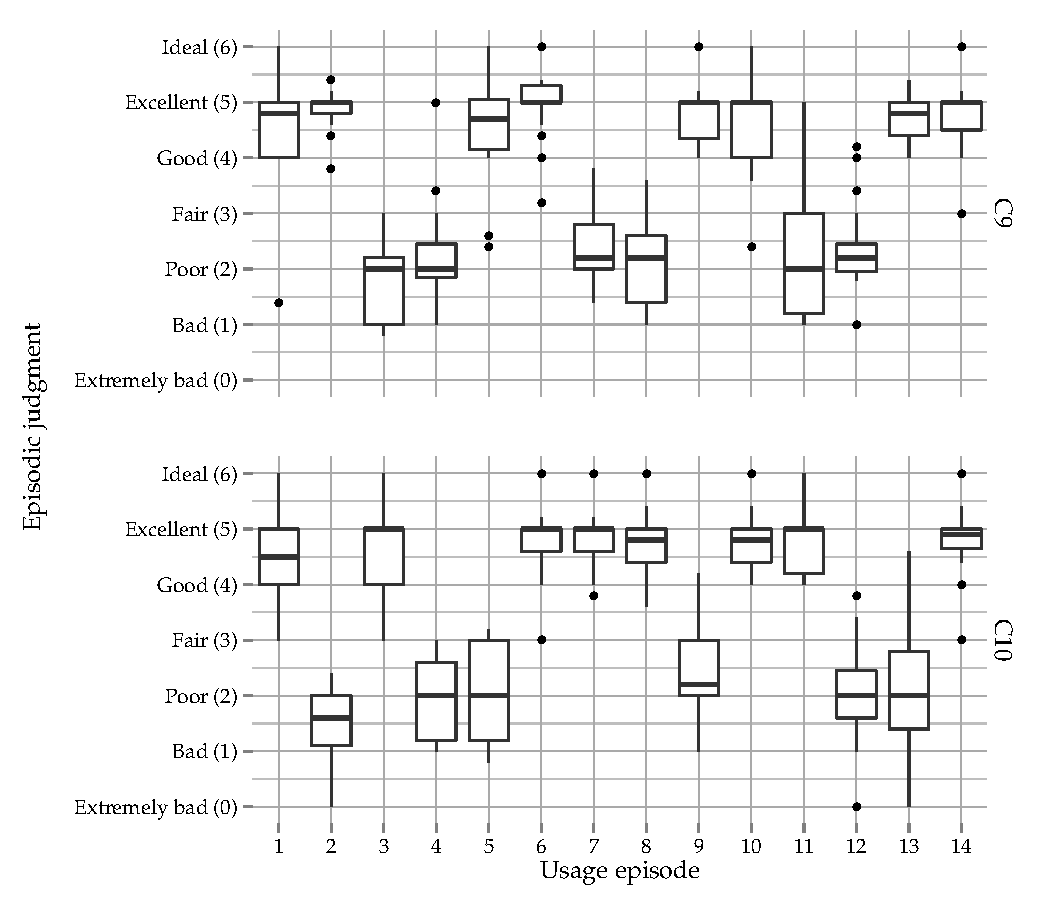
\includegraphics[width=\maxwidth]{figure/plotE5-1} 

\end{knitrout}
	\caption[Multiple days (\E5{}): box plots of episodic judgments for \C9{} and \CX{}]{Multiple days: box plots of episodic judgments in \E5{} for \C9{} (top) and \CX{} (bottom).}
	\label{img:field:boxplotE5}
\end{figure}

\paragraph*{Multi-episodic Judgments}
The multi\-/episodic judgments for both services and conditions are shown in \autoref{tab:field:e5results}.
For the \ac{AoD} service, no significant differences between multi\-/episodic judgments are observed for \C9{} ($H(4)=6.8676$, $p=0.1431$).
For \CX{}, a significant difference is found ($H(4)=10.2563$, $p=0.0363$).
However, a post-hoc test does not find significant differences for \CX{} ($p\geq0.055$). %$p=0.555$, $p=0.291$, $p=0.055$, $p=0.165$, $p=NA$, $p=1.000$, $p=1.000$, $p=1.000$, $p=NA$, $p=NA$, $p=1.000$, $p=1.000$, $p=NA$, $p=NA$, $p=NA$, $p=1.000$
For the \ac{AoD} service, comparing the multi\-/episodic judgments between the two conditions does not indicate large effects (see \autoref{tab:field:e5results}).

For the \ac{VoD} service, no significant differences between multi\-/episodic judgments are found for \C9{} ($H(4)=3.2427$, $p=0.5181$).
For \CX{}, significant differences are found ($H(4)=22.8848$, $p<0.001$).
A post-hoc test shows that the multi\-/episodic judgment of the 2nd~day is significantly different to all following multi\-/episodic judgments ($p<0.006$). %$p=0.002$, $p=0.002$, $p=0.003$, $p=0.005$, $p=NA$, $p=1.000$, $p=1.000$, $p=0.697$, $p=NA$, $p=NA$, $p=1.000$, $p=0.718$, $p=NA$, $p=NA$, $p=NA$, $p=1.000$
Between the two conditions, only the multi\-/episodic judgment of the 2nd~day is significantly different ($W=0.00$, $p<0.001$).

\begin{table}[t]
	\centering
	\caption[Multiple days (\E5{}): multi\-/episodic judgments]{Multiple days (\E5{}): multi\-/episodic judgments. Reported as \ac{MOS} with standard deviation in brackets.}
	\label{tab:field:e5results}
	\begin{tabularx}{\textwidth}{Y|Y|Y||Y|Y}
	Day & \multicolumn{4}{c}{Multi-episodic judgment} \\
	 			& \multicolumn{2}{c}{\ac{AoD}} & \multicolumn{2}{c}{\ac{VoD}} \\
 	& \C9{} & \CX{} & \C9{} & \CX{} \\
	\midrule
	2 & 4.0 (0.7) & 4.4 (0.8) & 3.7 (0.4) & 5.2 (0.3) \\
	\hline
	5 & 3.0 (0.7) & 3.7 (0.7) & 3.7 (0.4) & 3.4 (0.7) \\
	\hline
	8 & 3.6 (0.9) & 3.6 (0.6) & 3.9 (0.4) & 3.4 (0.9) \\
	\hline
	11 & 3.6 (0.8) & 3.3 (0.6) & 3.8 (0.4) & 3.5 (1.0) \\
	\hline
	14 & 3.6 (0.9) & 3.5 (0.6) & 3.5 (0.5) & 4.0 (0.7) \\
	\end{tabularx}
\end{table}

\subsection{Discussion}
In \E5{}, the implemented system was able to provide the desired performance levels in a reliable manner as reflected by the episodic judgments.
As long as only \ac{HP} episodes were presented, the following multi\-/episodic judgment remained on a similar level as the episodic judgments for both services (\CX{}).
This is in line with \citet{moller_single-call_2011} and also \E4{}.
It is notable that the episodic judgments are not very different between the two services.
A reason for this might be that both services presented the audio modality with the same codec configuration and thus similar degradations.

As desired, the presentation of \ac{LP} episodes affected the following multi\-/episodic judgments.
However, the two conditions resulted only in limited variation of multi\-/episodic judgments after the first \ac{LP} episode was presented.
Except for the first multi\-/episodic judgment of the \ac{VoD} service, no differences between the two conditions could be observed.
In \C9{}, even the presentation of three consecutive days in \ac{HP} indicated only a \emph{slight}, non-significant increase.
This suggests a longer integration interval for the multi\-/episodic judgments than three days, \ie, prior experiences still affected the judgments.
That no difference between the two conditions could be observed, indicates that the number of day-wise performance changes did not affect the multi\-/episodic quality formation process and thus suggests that \autoref{hypo:consecutive} is false.
%It must be noted that multi\-/episodic judgment remained on a similar level and did not decrease further towards episodic judgments of \ac{LP}.
%Thus, multi\-/episodic judgments tend to stay between episodic judgments for \ac{HP} and \ac{LP} without a tendency towards one of both.
%As only two conditions have been investigated in this experiment, a precise characteristic cannot be determined.
The results of \E5{} can be used for model verification only, as the two conditions yielded very similar results.

\section{Experiment E6}
\E6{} is a follow-up to the one-session experiments, but extends the usage period to 6~days with one usage episode per session.
The main goal of this experiment was to investigate if the effects observed in one session can also be observed in longer usage periods.
Besides interesting knowledge, this is an important aspect for the implementation of prediction models.
%If similar effects are observed, a prognosis model can be implemented that can be applied in both settings.
%If not, then individual prognosis models have to be developed or add the length of usage period as a parameter.
In \E6{}, a \ac{AoD} service is used to investigate a subset of the presented hypotheses (\cf{} \autoref{hypotheses}).
Here, the impact of the number of \ac{LP} episodes (\autoref{hypo:number}), the position of \ac{LP} episodes (\autoref{hypo:position}), and consecutive versus non-consecutive \ac{LP} episodes (\autoref{hypo:consecutive}) were investigated.

\subsection{Design}
The experimental design of \E6{} is similar to the one-session experiments.
On each of the 6~days, the \ac{AoD} service needed to be used twice per day.
%In this experiment, two different performance level were applied, \ie, \ac{HP} and \ac{LP}.
%\subsubsection{Conditions}
For the investigation of the three hypotheses, six multi\-/episodic conditions were created.
Here, the performance was varied on a per day basis, \ie, the two episodes of the same day were presented with the same performance level.
The multi\-/episodic conditions are similar to the one-session experiments and are thus denoted with the \emph{same} abbreviations (see \autoref{C0}).
In all conditions, the first three days were presented in \ac{HP}.
\ac{LP} episodes were only presented from the 4th~day to the 6th~day.
The conditions are \C1{}, \C3{}, \C4{}, \C5{}, \C6{}, and \C8{}.
\C1{} and \C3{} present either the 4th or the 6th~day in \ac{LP}.
\C4{}, \C5{}, and \C8{} present two days between the 4th and the 6th~day in \ac{LP}.
\C6{} presents all usage episodes on these three days in \ac{LP}.

For the investigation of \autoref{hypo:number}, the results of \C3{}, \C5{}, and \C6{} can be compared.
\autoref{hypo:position} can be evaluated by comparing the results of \C1{} and \C3{} as well as \C4{} and \C5{}.
Finally, \autoref{hypo:consecutive} is evaluated by comparing the results of \C8{} with \C3{} and \C5{}.
%\autoref{tab:field:e6episodic} gives an overview on the conditions and the number of participants.

As in \E3{} and \E5{}, the audio book \emph{City of the Beasts} from Isabel Allende was used.
In \E3{}, episodes with a duration of approximately \unit[3]{min} were used, whereas \E5{} used \unit[12..17]{min}.
For \E6{}, a duration of \unit[6..8]{min} was chosen.
This should enable participants to focus on the content while limiting their effort.
Again, the audio book was cut, so individual scenes were self-contained.
The scenes were presented in the chronological order (one scene per episode).

%\subsubsection{Feedback}
Before starting the 6~day usage period, an introductory session was conducted.
Here, participants received all necessary information about the experiment and demographic data was collected.
Then, participants were presented typical speech telephony degradations, \ie, training, in the same way as in the one-session experiments (\cf{} \autoref{sec:training}).
Finally, participants used the \ac{AoD} service for two episodes to ensure that they understood how to use the \ac{AoD} service.

During the multi\-/episodic part of this experiment, the first episode of a day needed to be conducted between \unit[7]{am} and \unit[1]{pm} and the second episode between \unit[3]{pm} and \unit[10]{pm}.
Episodic judgments and multi\-/episodic judgments were taken on the 7\=/point \ac{CoCR} scale.
Multi\-/episodic judgments were collected after the second episode of the 3rd~day and the 6th~day.
In fact, the judgment after the 3rd~day is thus only based on \ac{HP} episodes.
Thus, it can be used as reference point to assess the impact of the presented \ac{LP} episodes on the final multi\-/episodic judgment.
This is similar to the one-session experiments and in the following denoted also as \emph{reference}.
After each episode, two content-related questions were presented to force participants to pay attention to the content.
Here, the correct answer out of three options needed to be selected.
This allows to evaluate if participant had experienced an episode and thus could answer the questions correctly.

On the day after finishing the usage period, a final interview was conducted.
%In this interview the retrospective quality for every day, and the content answers for every episode were assessed.
Here, participants were interviewed about issues with the technical system.
%In addition, potential issues with the provided technical system were assessed.

In this experiment, participants used their own computer and their own pair of headphones.
Participants could access the \ac{AoD} service via the Internet using a \textsc{\lowercase{HTML5}}-capable web browser.
For \ac{HP}, the source material (\textsc{\lowercase{CD}}, \unit[44.1]{kHz}, stereo) was encoded with \ac{MP3} (\unit[192]{kbit/s}).
This was necessary to enable media distribution via Internet, as uncompressed audio data is not suited for this.
In fact, the bitrate was selected to produce no audible impairments for the used speech-only content.
For \ac{LP}, the content was first encoded with \textsc{\lowercase{LPC\=/10}} before encoding it finally with \ac{MP3}.
A detailed description of the implemented system is given in the \appendix{}~\ref{appendix:setups} (p.\,\pageref{appendix:setups}).

\subsection{Participants}
\E6{} was conducted in Berlin from September until November~2015.
Participants were required to have normal hearing capabilities.
This experiment was conducted with 57~female and 38~male participants aging from of 18~to~33~years ($\mu=25.8$, $\sigma=4.0$). %data=read.csv("#DataRaw/field-aod_data.csv"); data = data[-which(!data$Valid), ]
Participants received \unit[20]{\textsc{\lowercase{EUR}}} as compensation.
In this experiment, all usage episodes were conducted and all questionnaires filled.
Here, participants were informed by email, when a usage episode should be conducted, and a digital questionnaire system was used.



Similar to the laboratory experiments, each participant was individually checked for inconsistent episodic judgments.
A participant is considered inconsistent if more than two episodic judgments exceed the 1.5~$\times$ \emph{interquartile range} of the performance levels of this condition.
None of the participants fulfilled this criteria.
In addition, the content-related questions were evaluated.
Here, it was required that participants should answer at least 50\% of the questions correctly to assume they followed the experimental instructions.
Out of the 24~questions, participants answered on average 20.8 questions ($\sigma = 2.7$) correctly.
One participant who participated in \C8{} is excluded from data analysis, because only 8~questions were correctly answered.



\subsection{Data Analysis}
In the following, the data of \E6{} are analyzed.
First, the potential impact of the between-subject design is evaluated.
Then, the multi\-/episodic judgments are evaluated with regard to the three investigated hypotheses.

\subsubsection{Consistency}
An impact of the between-subject design is investigated by evaluating the episodic judgments of \ac{HP} and \ac{LP}.
\autoref{tab:field:e6episodic} shows the episodic judgments for all conditions.
A significant difference is found for \ac{HP} ($H(5)=33.4978$, $p<0.001$).
A post-hoc tests shows that \C5{} is significantly different to all other conditions ($p<0.05$). %wilcox.pairwise.print(QU~condition, "E6a", "HP"))
In addition, \C3 is significantly different to \C4{} and \C8{} ($p<0.02$).
For \ac{LP}, significant differences between conditions are also found ($H(5)=18.2748$, $p=0.0026$).
A post-hoc tests shows that \C5{} is significantly different to \C1{}, \C4{}, and \C8{} ($p<0.05$). %wilcox.pairwise.print(QU~condition, "E6a", "LP")
It must be noted that episodic judgments of \C5{} resulted in the highest \ac{MOS} for \ac{HP} and in the lowest \ac{MOS} for \ac{LP}.
A detailed analysis did not yield a reason for the difference, and it is thus considered an artifact due to the between-subject design.
Box plots for all conditions can be found in the \appendix{}~\ref{appendix:results} (p.\,\pageref{appendix:results}).

\begin{table}
	\centering
	\caption[Multiple days (\E6{}): overview on conditions]{Multiple days (\E6{}): overview on conditions. Reported as \ac{MOS} with standard deviation in brackets.}
	\label{tab:field:e6episodic}
	\begin{tabularx}{\textwidth}{Y|Y|Y|Y|Y}
	Condition & \ac{LP} days & Participants &  \ac{HP} & \ac{LP} \\
	\midrule
	\C1 & 4 		& 16 & 4.5 (0.9) 	& 1.3 (0.8) \\
	\hline
	\C3 & 6 		& 15 & 4.7 (0.7) 	& 1.3 (0.8) \\
	\hline
	\C4 & 4..5	& 14 & 4.5 (0.7)		& 1.3 (0.5) \\
	\hline
	\C5 & 5..6	& 18& 5.0 (0.8)	& 0.9 (0.5) \\
	\hline
	\C6 & 4..6	& 15	& 4.6 (0.6)		& 1.2 (0.7) \\
	\hline
	\C8	& 4 and 6	& 16 & 4.5 (0.6)		& 1.2 (0.7) \\
	\end{tabularx}
\end{table}

For the multi\-/episodic judgment after the 3rd~day, no significant differences between conditions are observed ($H(5)=5.2111$, $p=0.3907$).
This indicates that as long as only \ac{HP} episodes were presented, the between-subject design did not affect multi\-/episodic judgments.

\subsubsection{\autoref{hypo:number}: Number of \acs{LP} Episodes}
In \autoref{hypo:number}, it is assumed that increasing the number of \ac{LP} episodes before a multi\-/episodic judgment results in a decrease of this judgment.
This hypothesis can be evaluated by comparing the final multi\-/episodic judgment between the \emph{reference}, \C3{}, \C5{}, and \C6{}.
These present none, one, two, and three days in \ac{LP} before the multi\-/episodic judgment.
\autoref{tab:field:hyponumber} shows the final multi\-/episodic judgment and the reference for these conditions.

\begin{table}[t]
	\centering
	\caption[Multiple days (\E6{}): multi\-/episodic judgments after the 6th~day for \autoref{hypo:number}]{Multiple days (\E6{}): multi\-/episodic judgments after the 6th~day for \autoref{hypo:number}. Reported as \ac{MOS} with standard deviation in brackets.}
	\label{tab:field:hyponumber}
	\begin{tabularx}{\columnwidth}{Y|Y|Y}
	Condition	& \ac{LP} episode(s) 	& Multi-episodic judgment\\
	\midrule
	Reference	(\ac{HP} only) & - & 4.7 (0.6) \\
	\hline
	\C3{}			& 6				& 3.6 (0.6)\\
	\hline
	\C5{}			& 5..6			& 2.5 (1.0)\\
	\hline
	\C6{}			& 4..6			& 2.4 (0.7)\\
	\end{tabularx}
\end{table}

\C3{}, \C5{}, \C6{}, and the reference are significantly different ($H(3)=68.3657$, $p<0.001$).
A post-hoc test finds that the reference is significantly different to all three conditions ($p<0.001$).
In addition, \C3{} and \C5{} ($p=0.002$) as well as \C3{} and \C6{} are significantly different ($p<0.001$).
For \C5{} and \C6{}, no significant difference is found ($p=0.366$).

The results show that increasing the number of \ac{LP} days directly before the multi\-/episodic judgment results in a reduction of this judgment.
Here, a reduction of approximately \unit[1]{pt} for none to one and one to two days is observed.
However, no further decrease can be observed if three days are presented in \ac{LP}.
It must be noted that the multi\-/episodic judgment remains \unit[1]{pt} higher than the episodic judgments of \ac{LP} episodes.
With regard to \autoref{hypo:number}, the results are in line the one-session experiments \E1{} and \EIIa{}.
For both usage periods, the multi\-/episodic judgment decreases until two episodes/days were presented in \ac{LP}.
Then, the judgment remains on the same level above the episodic judgments of \ac{LP}.
Thus, \autoref{hypo:number} can only be partly accepted.
However, the underlying reason for the observed saturation could not be derived from this experiment.

\subsubsection{\autoref{hypo:position}: Position of \acs{LP} Episode(s)}
In \autoref{hypo:position}, it is assumed that presenting \ac{HP} episodes after \ac{LP} episodes reduces the negative impact on the directly following multi\-/episodic judgment.
This can be investigated for one day in \ac{LP} with \C1{} and \C3{} as well as for two days in \ac{LP} with \C4{} and \C5{}.
\autoref{tab:field:hypoposition} shows the final multi\-/episodic judgment for these four conditions.

\begin{table}[t]
	\centering
	\caption[Multiple days (\E6{}): multi\-/episodic judgment after the 6th~day for \autoref{hypo:position}]{Multiple days (\E6{}): multi\-/episodic judgment after the 6th~day for \autoref{hypo:position}. Reported as \ac{MOS} with standard deviation in brackets.}
	\label{tab:field:hypoposition}
	\begin{tabularx}{\columnwidth}{Y|Y|Y}
	Condition   & \ac{LP} episode(s) 	& Multi-episodic judgment \\
	\midrule
	\C1{}			& 4				& 4.1 (0.7)\\
	\hline
	\C3{}			& 6				& 3.6 (0.6)\\
	\hline
	\hline
	\C4{}			& 4..5			& 3.0 (1.1)\\
	\hline
	\C5{} 			& 5..6			& 2.5 (1.0)\\
	\end{tabularx}
\end{table}

With regard to the final multi\-/episodic judgment neither \C1{} and \C3{} ($W=138.50$, $p=0.136$, one-sided) nor \C4 and \C5 ($W=151.00$, $p=0.087$, one-sided) are significantly different.
Still, in both cases an effect of position is indicated and thus a recency effect might have been observed.
However, the results of \E6{} are inconclusive and thus \autoref{hypo:position} can neither be accepted nor be rejected.

\subsubsection{\autoref{hypo:consecutive}: Consecutive vs. Non-consecutive \acs{LP} Episodes}
In \autoref{hypo:consecutive}, it is assumed that consecutive \ac{LP} episodes yield a better multi\-/episodic judgment than the same number of \ac{LP} episodes presented non-consecutively.
This hypothesis can be evaluated by comparing \C4{} and \C5{} with \C8{}.
\C4{} and \C5{} present each two days \ac{LP} consecutively, whereas \C8{} presents the 4th and the 6th~day in \ac{LP}.
\autoref{tab:field:hypoconsecutive} shows the final multi\-/episodic judgment for these conditions.
These three conditions are not significantly different with regard to the final multi\-/episodic judgment ($H(2)=2.3809$, $p=0.3041$).

\begin{table}[b]
	\centering
	\caption[Multiple days (\E6{}): multi\-/episodic judgment after the 6th~day for \autoref{hypo:consecutive}]{Multiple days (\E6{}): multi\-/episodic judgment after the 6th~day for \autoref{hypo:consecutive}. Reported as \ac{MOS} with standard deviation in brackets.}
	\label{tab:field:hypoconsecutive}
	\begin{tabularx}{\textwidth}{Y|Y|Y}
	Condition   & \ac{LP} episode(s) 	& Multi-episodic judgment \\
	\midrule
	\C4{}			& 4..5			& 3.0 (1.1)\\
	\hline
	\C8{}			& 4 and 6	& 2.7 (0.4)\\
	\hline
	\C5{}			& 5..6			& 2.5 (1.0)\\
 \end{tabularx}
\end{table}

Thus, \autoref{hypo:consecutive} must be rejected, because no significant difference is observed.
It must thus be concluded that the non-consecutive case is judged not different than the consecutive case.
In fact, the slight improvement in the multi\-/episodic judgment of \C8{} compared to \C5{} can also be explained by a recency effect due to the earlier presentation of the first \ac{LP} episodes.
This observation is similar to \EIIa{}.

\subsection{Discussion}
In this experiment, three hypotheses were investigated complementing the one-session experiments.
In fact, an absolute comparison between \E6{} and the one-session experiments cannot be conducted due to the differences in the experimental designs.
Nevertheless, in \E6{} similar effects could be observed or were indicated.

For \autoref{hypo:number}, a decrease in the final multi\-/episodic judgment could be observed if up to two days were presented in \ac{LP}.
Presenting three consecutive days in \ac{LP} did not result in a further decrease.
This closely resembles the findings of \E1{} and \EIIa{}.

With regard to varying the position of one or two days in \ac{LP}, a recency effect is indicated (\autoref{hypo:position}).
For both cases, a (non-significant) increase of the multi\-/episodic judgments is indicated if \ac{HP} episodes are presented directly before the final judgment.
This is in line with the findings of \E1{} and partly with \EIIa{}.
In the latter, no effect could be observed for one \ac{LP} episode but for two consecutive \ac{LP} episodes.

\autoref{hypo:consecutive} must be rejected based on \E6{}.
Similar to \EIIa{}, the final multi\-/episodic judgment remains rather close.
The slight difference that is indicated between the conditions could also be explained by a recency effect.
In fact, this might even be an anomaly due to the between-subject design.
It must be concluded that increasing the number of performance level changes did not produce an observable effect.

\section{Conclusion}
\E6{} was conducted based on the practical knowledge gained in \E4{} and \E5{}.
\E4{} and \E5{} showed that multi\-/episodic perceived quality can be investigated in field experiments by applying the defined-use method.
Although the results were very limited, it was found that a media\-/on\-/demand service can be set up in a reliable manner.
Besides avoiding technical complexity, also employing pairs of participants has been found difficult in a field experiment (\E4{}).
Especially, the effort for each pair of participants to conduct the episodes together seems to be limiting.
These limitations could be overcome by using media\-/consumption tasks.
In addition, this allows to avoid the impact of varying user behavior on the duration of usage episodes.
This lead to the design of \E6{}.
This experiment was also inspired by the one-session experiments.
%This experiment could be conducted with a larger number of participants in a rather short period.
%Most important here, was that participants used their own hardware only.

For \autoref{hypo:number}, very similar results to the one-session experiments were observed.
A decrease in the final multi\-/episodic judgment could be observed if more \ac{LP} episodes were presented.
In addition, also an effect of saturation could be observed.
This indicates that the integration interval of the formation process is longer than 3~days, as previous \ac{HP} episodes still affected the final multi\-/episodic judgment.
With regard to \autoref{hypo:position}, \ie, impact of varying position of \ac{LP} episodes, an effect is indicated (non-significant).
Here, a recency effect seems to occur.
This is line with the results of \E1{} and \EIIa{}.

With regard to \autoref{hypo:consecutive}, the results are similar to \EIIa{}.
Here, no significant difference is observed between the non-consecutive and consecutive presentation of two \ac{LP} days.
The indicated difference might also be attributed to a recency effect.
Thus, the non\-/consecutive presentation seems to be judged similar to the consecutive presentation or the effect size seems to be rather small.
Therefore, \autoref{hypo:consecutive} must be rejected.

It must be noted that in \E6{} effects were observed or indicated that are similar to the one-session experiments.
This indicates that the presentation of episodes itself has a higher impact on the quality formation process than the actual time between episodes.
However, a direct comparison of the results of these experiments cannot be conducted due to the differences in the experimental designs, \ie, tasks, service types, and duration of usage episodes.

In difference to \E4{} and \E5{}, \E6{} provides a large data set (6~conditions, 95~participants).
In the following chapter, this data set forms the basis for the development and the evaluation of models for the prediction of multi\-/episodic judgments based on episodic judgments.


%OPTIONAL!
%\section{Digression: On practical aspects of Field Studies}
%\begin{itemize}
%\item Production Ready Systems
%\item Temporal Constraint
%\item "Real" environment (subject's own context)
%\item Cheater detection for consumption only
%\item Drop out rate
%\end{itemize}
